\chapter{Performantie}
\label{app:performantie}

In deze appendix wordt een gedetailleerd overzicht gegeven van de performantie voor de vier raamwerken op de acht apparaten: 
\st{} (zie \ref{sec:app-performantie-st}),
\kendo{} (zie \ref{sec:app-performantie-kendo}),
\jqm{} (zie \ref{sec:app-performantie-jqm}),
\lungo{} (zie \ref{sec:app-performantie-lungo}).

%%%%%%%%

\section{\st}
\label{sec:app-performantie-st}
Op figuur~\ref{fig:performantie-st} worden de gemiddelde downloadtijd van \st{} getoond op elk apparaat.0.75

\begin{figure}
  \centering
  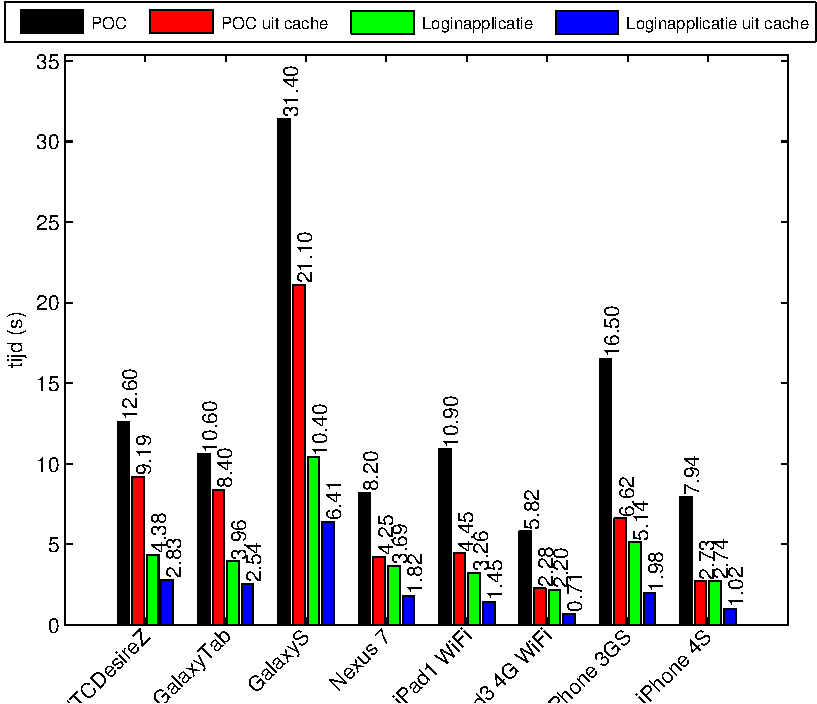
\includegraphics[width=0.8\textwidth]{figuren/performance-st.pdf}
  \caption{Gemiddelde downloadtijden van \st{} voor POC,  POC uit cache,  Login en Login uit cache voor elk apparaat.}
  \label{fig:performantie-st}
\end{figure}

Voor de POC is een dalende downloadtijd waarneembaar wanneer het Android-apparaat recenter wordt.
De downloadtijd van de POC op de \gs{} duurde gemiddeld $31.43$s!
Gemiddeld moeten Android toestellen $5$ seconden langer laden in vergelijking met iOS toestellen.
Dit gemiddelde wordt sterk beinvloed door de trage laadtijd van de \gs{}.

\st{} heeft een andere aanpak voor het cachen van een applicatie door de introductie van een \term{Delta-update} mechanisme.
Dit mechanisme wil voorkomen dat bij een kleine aanpassing in de code,  alle bestanden opnieuw moeten worden opgehaald die in het \term{manifest} bestand staan opgelijst.
De \term{Micro-loader} is verantwoordelijk voor het asynchroon ophalen van all benodigde \js{}- en CSS-bestanden.
Na het bouwen van een applicatie met Sencha Cmd,  zullen de gewijzigde bestanden gearchiveerd worden en worden de veranderingen tussen elke versie opgeslagen.
Na het laden van de applicatie, zal de \code{Micro-loader} met een GET-verzoek controleren op wijzigingen.
Dit GET-verzoek zal de grootste tijd voor zijn rekening nemen bij de laadtijden bij applicaties uit de cache.
\st{} heeft er dus voor gekozen om aan performantie in te boeten ten voordele van het update mechanisme.
%TODO referentie http://www.sencha.com/blog/behind-sencha-command-and-the-build-process


Een laatste opmerking die bij \st{} moet worden gemaakt, is dat AJAX-verzoeken van een \code{proxy} naar een ander domein altijd vooraf worden gegaan met een OPTIONS-verzoek.
Dit is een verzoek om informatie over de beschikbare opties van het communicatiekanaal op te vragen.
Standaard zet \st{} de \code{X-Requested-With} op XMLHttpRequest en hierdoor zal de browser een OPTIONS-verzoek als \term{preflight} sturen.
%Setting custom headers on XHR requests triggers a preflight request. %http://remysharp.com/2011/04/21/getting-cors-working/
%http://stackoverflow.com/questions/10236056/when-loading-a-store-in-sencha-touch-2-how-can-i-stop-the-additional-options-ht
% POST /resources/userService/login?_dc=1368367749599 HTTP/1.1
% Host: kulcapexpenseapp.appspot.com
% Connection: keep-alive
% Content-Length: 54
% Origin: http://sandervanloock.github.io
% User-Agent: Mozilla/5.0 (X11; Linux i686) AppleWebKit/537.11 (KHTML, like Gecko) Chrome/23.0.1271.64 Safari/537.11
% Content-Type: application/x-www-form-urlencoded; charset=UTF-8
% Accept: */*
% Referer: http://sandervanloock.github.io/HTMobieL/Sencha/build/ExpenseApp/production/index.html
% Accept-Encoding: gzip,deflate,sdch
% Accept-Language: nl-NL,nl;q=0.8,en-US;q=0.6,en;q=0.4
% Accept-Charset: ISO-8859-1,utf-8;q=0.7,*;q=0.3
% 
% Accept:*/*
% Accept-Charset:ISO-8859-1,utf-8;q=0.7,*;q=0.3
% Accept-Encoding:gzip,deflate,sdch
% Accept-Language:nl-NL,nl;q=0.8,en-US;q=0.6,en;q=0.4
% Connection:keep-alive
% Content-Length:23
% Content-Type:application/x-www-form-urlencoded; charset=UTF-8
% Host:kulcapexpenseapp.appspot.com
% Origin:http://sandervanloock.github.io
% Referer:http://sandervanloock.github.io/HTMobieL/Sencha/build/ExpenseApp/production/index.html
% User-Agent:Mozilla/5.0 (X11; Linux i686) AppleWebKit/537.11 (KHTML, like Gecko) Chrome/23.0.1271.64 Safari/537.11
% X-Requested-With:XMLHttpRequest

%%%%%%%%

\section{\kendo}
\label{sec:app-performantie-kendo}
Op figuur~\ref{fig:performantie-kendo} worden de gemiddelde downloadtijd van \kendo{} getoond op elk apparaat.

\begin{figure}
  \centering
  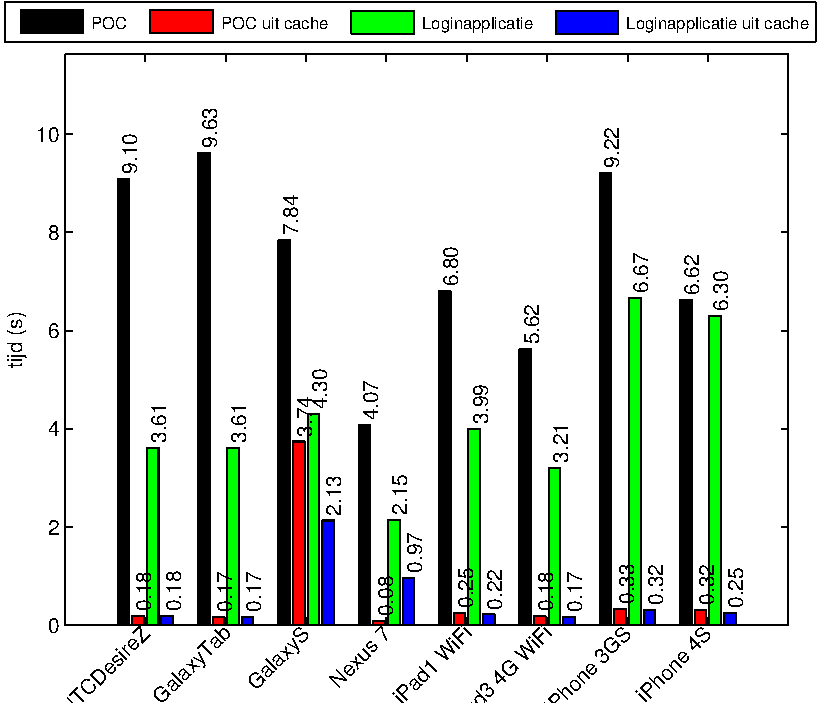
\includegraphics[width=0.8\textwidth]{figuren/performance-kendo.pdf}
  \caption{Gemiddelde downloadtijden van \kendo{} voor POC,  POC uit cache,  login en login uit cache voor elk apparaat.}
  \label{fig:performantie-kendo}
\end{figure}

De \gtab{} vertoond de hoogste laadtijd,  gevolgd door de \iphoneiii{} en \htc.
Opmerkelijk is dat de gecachete versie van de loginapplicatie op de \nexus{} $10$ keer trager laadt dan de gecachete versie van de POC.
Het ophalen van een gecachete applicatie werkt bij de \gs{} het traagst.

Bij \kendo{} is er geen opmerkelijk verschil waarneembaar tussen Android en iOS toestellen (Android gemiddeld slechts $60$ms trager).

%%%%%%%%

\section{\jqm}
\label{sec:app-performantie-jqm}
Op figuur~\ref{fig:performantie-jqm} worden de gemiddelde downloadtijd van \jqm{} getoond op elk apparaat.

\begin{figure}
  \centering
  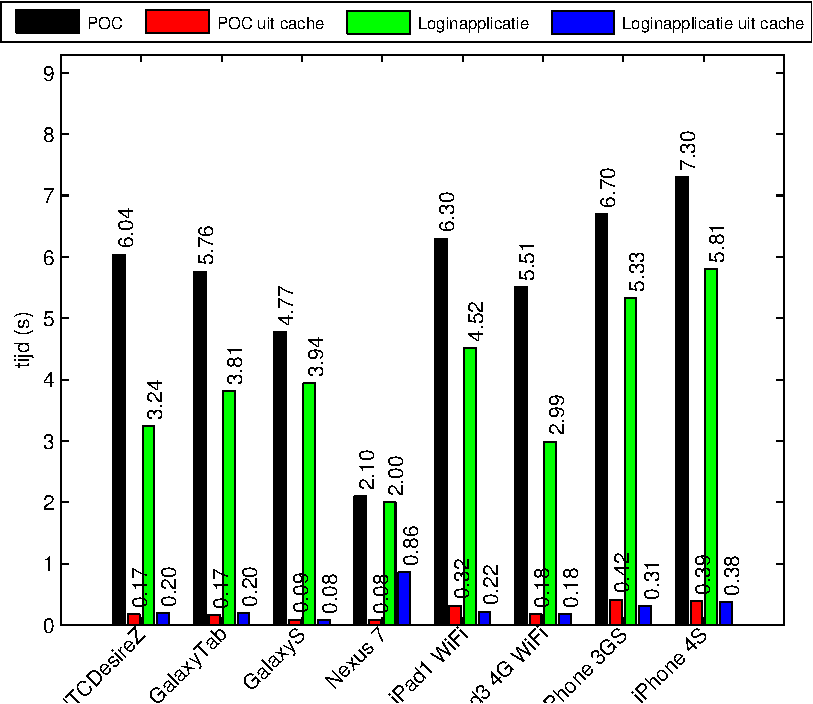
\includegraphics[width=0.8\textwidth]{figuren/performance-jquery.pdf}
  \caption{Gemiddelde downloadtijd van \jqm{} voor POC,  POC uit cache, login en login uit cache voor elk apparaat.}
  \label{fig:performantie-jqm}
\end{figure}

%TODO Sander: fout (\gs is minst recent...
Voor de POC is een dalende downloadtijd waarneembaar wanneer het Android-apparaat recenter wordt.
Dit is echter ook zo voor de iPads van Apple, maar voor de iPhones stijgt de downloadtijd.
Er zijn minimale verschillen bij de gecachete versie van de POC, waarbij het het langste duurt op de \ipadi{}.

Als de loginapplicatie wordt bekeken, wordt hetzelfde waargenomen als voor de POC.
Enkel bij de Android-apparaten wordt de downloadtijd trager, naarmate het toestel recenter wordt.
Dit is in tegenstelling tot de POC.

Een opmerkelijke waarneming is dat het langer duurt om de gecachete versie van het loginscherm te laden dan de volledige POC.

%%%%%%%%

\section{\lungo}
\label{sec:app-performantie-lungo}

\begin{figure}
  \centering
  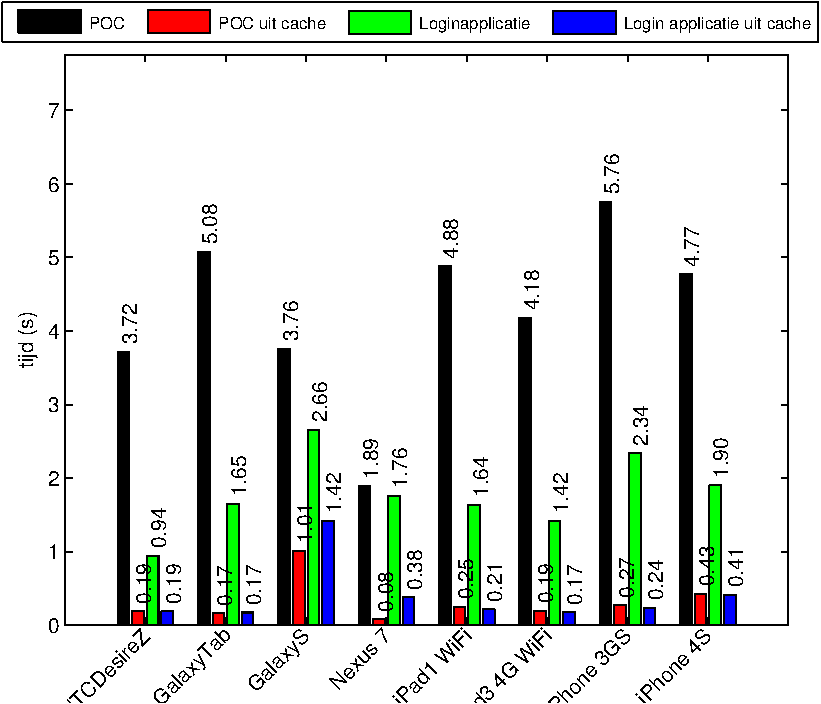
\includegraphics[width=0.8\textwidth]{figuren/performance-lungo.pdf}
  \caption{Gemiddelde downloadtijd van \lungo{} voor POC,  POC uit cache,  Login en Login uit cache voor elk apparaat.}
  \label{fig:performantie-lungo}
\end{figure}

%%% Local Variables: 
%%% mode: latex
%%% TeX-master: "masterproef"
%%% End: 
